\chapter{Introduction}
\section{Introduction générale}
%Il y sera question de présenter les enjeux des thématiques abordées ainsi que les objectifs recherchés à travers ce mémoire%
 Ce mémoire détaillera la conception d’un système dont l’objectif est de cartographier la ville de Douai à l’époque du XIIIe siècle sur la base de fouilles de texte automatisées à travers un registre de rentes d'époque, celui de Jehan de France, un riche marchand drapier et patricien de la ville de Douai. Trois thèmes majeurs des sciences de l'information et de la communication seront au centre de cette recherche :
 
 La première thématique est l’application des outils de traitement automatique des langues naturelles (TALN) aux textes historiques. L’émergence des humanités numériques a ouvert la recherche en sciences humaines à de nouvelles méthodes d’analyses qui ont, depuis, déjà grandement prouvées leur efficacité. Cependant, dans le cadre de l’étude de textes historique les outils utilisés par celles-ci se heurtent à de lourdes complications. L’une des principales est le langage dans lequel sont écrits des textes historiques : les outils de fouilles de textes sont généralement conçus pour traiter les langues très représentées telles que l’anglais ou le français et non des langues anciennes. Pour cause, une grande partie de ces outils ont besoin de corpus de textes conséquent ou de dictionnaires pour être performants. Un facteur accentuant cet état de fait est qu’il est relativement compliqué de composer un corpus de textes historiques : d’une part, car les textes anciens, étant sur des supports physiques, doivent être numérisés et ocrisés avant de pouvoir être utilisés, et d’autre part, car les sources écrites sont régulièrement lacunaires ou amputées d’une partie de leur contenu. La personne cherchant à traiter de façon automatisée des textes historiques devra donc se montrer créative.
 
La seconde thématique est l’application de la théorie des graphes au domaine de l’Histoire. La théorie des graphes trouve ses premières origines dans les travaux du mathématicien Leonhard Euler en 1735 et son problème des « sept ponts de Königsberg ». Les graphes permettent de modéliser des problèmes complexes sous la forme d’une structure de sommets reliés entre eux par des arêtes où les sommets renvoient à des référents — cela peut être des personnes, des lieux, des propositions, etc. — et les arêtes aux relations qui les relient entre eux. Si la théorie fut d’abord utilisée pour résoudre des problèmes de géométrie ou de mathématique, elle s’est popularisée dans le domaine des sciences humaines dans les années 1960 afin de modéliser diverses problématiques.

Finalement, la troisième thématique est celle de la visualisation des données sous forme de cartographies. L’intérêt de la cartographie dans la recherche en Histoire est multiple. Le premier est que ces cartes sont la représentation d’un grand nombre de données agrégées. Elles permettent donc d’analyser des phénomènes déjà connus d’un point de vue plus éloigné et plus global, permettant ainsi de découvrir de nouvelles relations corollaires ou causales entre différents évènements qui ne semblaient pas forcément liés aux premiers abords. À l’instar de l’exploration de graphiques et données statistiques, l’exploration des différents types de cartes se pose comme une approche complémentaire à l’étude des sources primaires dans les recherches en Histoire.

Un autre intérêt majeur de la visualisation des données se trouve dans la communication et la transmission des savoirs. En effet, l’information visuelle, pour peu qu’elle soit correctement organisée et présentée, s’appréhende et s’assimile avec plus d’aisance que l’information textuelle brute. Or c’est dans cette transmission que l’étude de l’Histoire prend son plein sens.

\section{Question de recherche}
 La question de rechercher est "La théorie des réseaux, appliquée au domaine des patrimoines immobiliers en Flandre médiévale, couplée à une fouille de texte automatisée dans des textes historiques, permet-elle de produire des visuels cartographiques pertinents à l’étude de l’histoire urbaine ?"
 
 Derrière cette question de recherche très vaste, se cache en réalité l'évaluation du résultat de trois objectifs distincts mis bout à bout : développer des algorithmes de fouille et traitement de texte adaptés à un document historique, appliquer la théorie des réseaux aux résultats de cette fouille afin de représenter des liens de mitoyenneté et finalement, transposer ces graphes en un visuel cartographique afin d'ouvrir de nouvelles voies de recherche dans l'étude du développement urbain.
 
\section{Hypothèse}
Le mémoire présente un travail de recherche et la conception d'un \textit{proof of concept} afin de répondre à la question de recherche. Très peu de travaux, si ce n'est aucun, n'ont été publiés sur cette méthode d'analyse des documents médiévaux. Il est donc difficile d'émettre des hypothèses quant aux limites que nous rencontrerons et sur les résultats que nous obtiendrons avec celle-ci.

Toutefois, cette méthode semble réalisable sur le papier et dans une optique optimiste,  les visuels produit devrait permettre de rendre compte des propriétés immobilières de Jehan de France, de la disparité et du types des loyers en fonction des quartiers de la ville, de la dispersion des noms de familles, etc. Des éléments qui, croisés  à d'autres sources, pourrait valider ou invalider d'autres hypothèses. 

\section{Contexte historique}
\subsection{La ville de Douai au XIIIe siècle}

Douai trouve ses origines au sixième siècle sur un îlot de la Scarpe (\cite{mestayer_douai_2016}), une rivière traversant le nord de la France et se déversant dans le fleuve de l'Escaut. Les terres fertiles des alentours offrent une rapide croissance à ce qui n'est alors encore qu'une petite agglomération rurale. Dès le Xe siècle, l'agglomération s'étend sur les rives de la Scarpe. Au Nord, sur la rive gauche de la rivière, le \textit{Duaculum}, appelé aussi le \textit{Douayeul}, une zone rurale dépendant de l'église Saint-Albin comprenant élevages de bêtes, greniers et brasseries (\cite{mestayer_douai_2016}). Sur l'autre rive, au Sud, le \textit{Castel Bourgeois}, un quartier qui s'oriente davantage vers le commerce et l'artisanat. Ce dernier deviendra la première place marchande de la ville (\cite{officedutourisme_douai_2016}, \cite{netteghem_histoire_2021}). En 967, Douai, qui à cette époque est encore appelé \textit{Castrum Duacum}, se dote d'une place-forte ainsi que d'une première muraille entourant la partie haute et basse de la ville (\cite{mestayer_douai_2016}). 

Forte de son activité agricole et de ses accès fluviaux, la ville gagna en richesse et devint un centre de commerce important dans la région, attirant marchands et artisans(\cite{clisant_vie_2003}). Les quartiers de la ville s'organisent alors en fonction des corporations d'artisans et marchands. On retrouve par exemple la rue des ferronniers, des foulons ou encore des bouchers. Les rues et places prennent à cette époque, où le pragmatisme  prévaut, une dénomination en fonction de leurs usages \cite{colin_decouvrez_2001}). 

Au XVIIe siècle, la disparité entre les deux rives se fait de plus en plus clivante et donne l'impression d'une ville séparée en deux entités distinctes (\cite{leroy-langelin_quartier_2012}). 
Le centre névralgique de la ville se consolide sur la rive droite de la Scarpe : une seconde enceinte, comportant douze portes, est édifiée afin d'englober l'expansion des quartiers autour du \textit{Castel bourgeois}, où des places de marchés ainsi que des halles apparaissent. 
Si le commerce céréalier fit démarrer la machine économique de la cité, Douai se forge maintenant une réputation, principalement, autour du commerce de draperies. Grâce aux foires de Champagne, la draperie Douaisienne s'exporte à travers à toute l'Europe, et même au delà (\cite{clisant_vie_2003}). Ce succès provient de la qualité et de la finition des étoffes produites, foulées aux pieds pour les plus précieuses. Chaque étape de la fabrication était supervisée par une des grandes familles bourgeoise de Douai (\cite{clisant_vie_2003}).
La progression économique qu'à connu la ville grâce au commerce de draperies était très liée à la production agricole des campagnes avoisinantes car ces dernières fournissaient la matière première à cette nouvelle industrie.
Cependant rapidement, la production de laine locale ne suffit plus à combler la demande en étoffes et un commerce s'installa avec l'Angleterre qui approvisionna alors Douai en laine(\cite{clisant_vie_2003}).

A la fin du XXIIe siècle, un premier échevinage apparaît, constitué de douze riches et notables douaisiens (\cite{mestayer_douai_2016}. Ceux-ci régissent les activités, ainsi que les affaires financières, policières et juridiques  de la ville au moyens de bans : une forme d'arrêté législatif (\cite{officedutourisme_douai_2016}). Ceci témoigne de la place, de plus en plus importante, qu'occupe les grandes familles bourgeoise dans l'administration et le développement de la ville.

Au cours de l'Histoire, Douai ne cessa d'être, tantôt Française, tantôt Flamande. Cependant, la richesse et la puissance de la ville, fît  qu'elle garda toujours une certaine indépendance vis à vis du rois de France ou du Compte de Flandre dans l'administration de sa cité (\cite{mestayer_douai_2016}).

La construction d'un nouveau rempart est entrepris au XIIIe siècle, justifié par l'apparition de nouveaux quartiers extérieur à la seconde enceinte, tel que la \textit{Neuville} au  Nord ou le \textit{Faubourg de Notre-Dame} à l'Est (\cite{netteghem_histoire_2021}).
Parallèlement à l'apogée économique de la ville, une nouvelle forme de capitalisation émerge : l'hiterage, qui recouvre toutes les formes de la propriété bâtie, y compris les terrains et les rentes de celles-ci. Ces bourgeois, principalement marchands et disposant déjà d'un certain capital mobilier, cherchent alors à acquérir biens-fonds et rentes ; un patrimoine qui devient un gage d'honorabilité et un signe de réussite dans la cité  (\cite{leguay_propriete_1989}). 


\begin{figure}[ht] % insère une figure ici (h = "here")
    \centering
    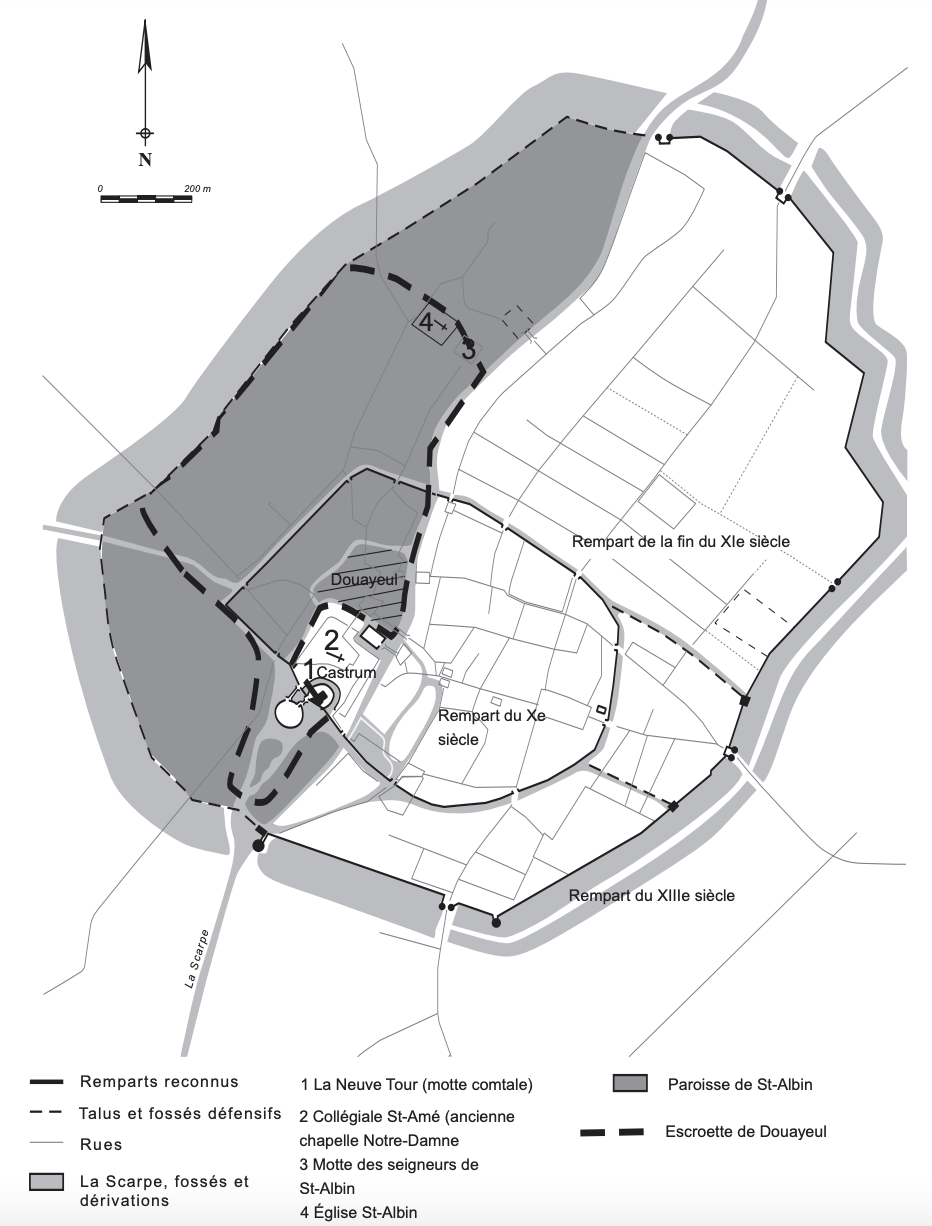
\includegraphics{1.Introduction/Img/Plan général de la ville de Douai avec les enceintes successives. DAO : E. Leroy-Langelin.png} 
    \caption{Plan général de Douai au XIIe s., E.Leroy-Langelin}
\end{figure}


\subsection{Sire Jean de France}
Sire Jean de France, ou Jehans de Franche, est un bourgeois notable de Douai : marchand drapier et un patricien de la seconde moitié du  XIIIe siècle.
Malgré son titre d'échevin de Douai et son patrimoine estimé à 316 rentes sur 529 maisons , ainsi que quelques propriétés hors de la ville (\cite{blockmans_trois_1941}), on retrouve finalement, assez peu de documentation ce personnage.

Si le régime patricien fut caractérisé par une exploitation de la misère, principalement des ouvriers et des universitaires, dont la figure la plus emblématique semblerait être Jehan Boinebroke. 
\quote 
    \og J. Boinebroke apparaît comme l'incarnation d'un capitalisme tellement hideux, si cruel et si impitoyable, que même la première moitié du xixe siècle n'en a pas connu de pareil ! \fg{} 
    \footnote{ Blockmans Fr. "Trois patriciens douaisiens de la seconde moitié du XIIIe siècle" In: Revue belge de philologie et d'histoire, tome 20, fasc. 1-2, 11941. p.266} 
\endquote
\vspace{0,5cm}
A son opposition, Jean de France est dépeint par G. Espinas et Fr. Blockmans comme un investisseur prudent et vertueux.
\subsection{Registre de rentes des propriétés foncières de Jean de France}
%Cette partie traitera de l’origine du carnet de rentes, de la façon dont sont agencées les informations et des données qu’il contient et que l’on cherche à extraire.%

